\documentclass{beamer}
\usepackage{../tut-slides}
\usepackage{../mathoperatorsAuD}

\usepackage{lmodern}
\usepackage{amsmath,amssymb}
\usepackage{wasysym}
\usepackage{stmaryrd}
\usepackage{enumerate}
%\usepackage[inline]{enumitem} 		%customize label
%\newcommand{\labelitemi}{\raisebox{1pt}{\scalebox{.9}{$\blacktriangleright$}}}
%\newcommand{\labelitemii}{$\vartriangleright$}
%\newcommand{\labelitemiii}{--}
\setbeamertemplate{itemize item}{\raisebox{1pt}{\scalebox{.9}{$\blacktriangleright$}}}
\setbeamertemplate{itemize subitem}{$\vartriangleright$}

\usepackage{booktabs}
\usepackage{tabularx}
\usepackage{tabu}
\newcommand*\head{\rowfont{\bfseries}}
\newcommand*{\tw}{\rowfont{\ttfamily}}
\renewcommand{\tabularxcolumn}[1]{>{\hspace{0pt}}m{#1}}
\usepackage{multirow}

\usepackage{tikz}
\usetikzlibrary{positioning, arrows, arrows.meta}
\usepackage{cancel}

\usepackage{empheq}
\newcommand*\widefbox[1]{\fbox{\hspace{2em} #1 \hspace{2em}}}

\usepackage{tcolorbox}
\newtcolorbox{mymathbox}[1][]{colback=white, sharp corners, #1}

\usepackage{xcolor}
\usepackage{listings}
\usepackage{bold-extra}
\newcommand*{\ttfamilywithbold}{\fontfamily{lmtt}\selectfont}
\lstset{numbers=left, 
	numberstyle=\tiny, 
	breaklines=true,
	backgroundcolor=\color{cdgray!20},
	numbersep=5pt,
	language=C,
	tabsize=2,
	basicstyle=\footnotesize\ttfamilywithbold,
	showstringspaces=false} 

\lstdefinestyle{notebook}{
	basicstyle=\footnotesize\ttfamilywithbold,   
	breakatwhitespace=false,         
	breaklines=true,                 
	commentstyle=\itshape, 
	escapeinside={\%*}{*)},          % if you want to add LaTeX within your code
	extendedchars=true,              % lets you use non-ASCII characters; for 8-bits encodings only, does not work with UTF-8
	backgroundcolor=\color{cdgray!10},
	frame=single,
	keywordstyle=\bfseries,       % keyword style
	morekeywords={}, 
	language=C,                 % the language of the code
	numbers=left,                    % where to put the line-numbers; possible: (none, left, right)
	numbersep=5pt,                   
	numberstyle=\tiny\color{cdgray!50}, 
	rulecolor=\color{cddarkblue}, 
	tabsize=2,
	frameround=tttt
}

\usepackage{MnSymbol}

\newcommand{\col}[1]{\textcolor{cdpurple}{#1}}
\newcolumntype{R}[1]{>{\centering\arraybackslash}p{#1}}
\usepackage{tabularx}
\renewcommand{\tabularxcolumn}[1]{m{#1}}

\usepackage{qtree}
\usepackage[edges]{forest}

\newcommand{\lefttree}{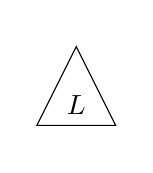
\begin{tikzpicture}
	\draw (0,0) node[anchor=north]{}
	-- (1,0) node[anchor=north]{}
	-- (.5,1) node[anchor=south]{}
	-- cycle;
	\draw (.5,.5) node[anchor=north]{$L$};
	\end{tikzpicture}}
\newcommand{\righttree}{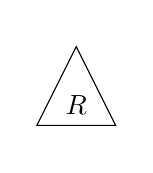
\begin{tikzpicture}
	\draw (0,0) node[anchor=north]{}
	-- (1,0) node[anchor=north]{}
	-- (.5,1) node[anchor=south]{}
	-- cycle;
	\draw (.5,.5) node[anchor=north]{$R$};
	\end{tikzpicture}}


\begin{document}	
	\title{Algorithmen und Datenstrukturen}
	\subtitle{Übung 9: AVL-Bäume \& Topologisches Sortieren}
	\author{Eric Kunze}
	\email{eric.kunze@tu-dresden.de}
	\city{TU Dresden}
%	\institute{Lehrstuhl für Grundlagen der Programmierung}
	\titlegraphic{\includegraphics[width=2cm]{../TUD-white.pdf}}
	\date{\formatdate{6}{12}{2021}}



%%%%%%%%%%%%%%%%%%%%%%%%%%%%%%%%%%%%%%%%%%%%%%%%%%%%%%%%%%%%%%%%%%%%%%%%%%%%%


\begin{frame}[fragile] \frametitle{Erinnerung: Bäume}
	\begin{lstlisting}[style=notebook]
typedef struct node *tree;
struct node { int key; tree left, right; };
	\end{lstlisting}

	\begin{minipage}{\dimexpr0.5\linewidth-\fboxrule-\fboxsep}
		\begin{tikzpicture}[%
			>=stealth',
			semithick,
			every node/.style={font=\scriptsize},
			inbox/.style={anchor=mid, font=\scriptsize, align=center, pos=0.5},
			]
			\draw[thick, rounded corners=2pt, color=cdpurple] (0,0) rectangle ++(2,1);
			\node[anchor=west, color=cdpurple] (struct node) at (2.05, 0.25) {\texttt{struct node}};
			\draw (0,0.5) -- (2,0.5)
			(1,0) -- (1,0.5);
			\path (0,0.5) rectangle ++(1,-0.5) node[inbox] (leftbox) {\texttt{left}} 
			rectangle ++(1, 0.5) node[inbox] (rightbox) {\texttt{right}}
			rectangle ++ (-2,0.5) node[inbox] {\texttt{key}};
			
			\draw[->, thick, color=cdblue] (1, 1.75) -- node[pos=0.2, right]{\texttt{tree t}} (1, 1);
			
			\draw[->, thick] (0.5,0) -- ++(-0.5,-0.75);
			\draw[->, thick] (1.5,0) -- ++( 0.5,-0.75);
			\node at (0,-1) {$\vdots$};
			\node at (2,-1) {$\vdots$};	
			
			\onslide<2->{%
				\draw[->, thick, color=cdgray] (0,1.75) --node[pos=0, above]{\texttt{tree* tp}} (1,1.75);
			}	
		\end{tikzpicture}
	\end{minipage}
	\pause\pause
	\begin{minipage}{\dimexpr0.5\linewidth-\fboxrule-\fboxsep}
		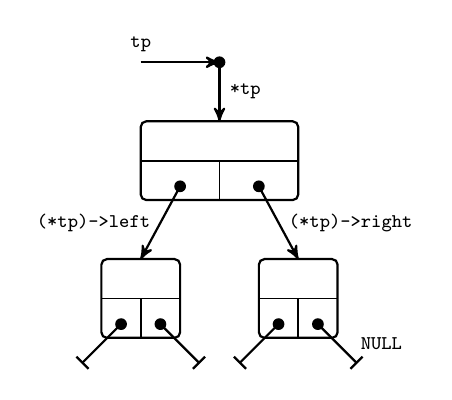
\begin{tikzpicture}[%
			>=stealth',
			semithick,
			every node/.style={font=\scriptsize},
			inbox/.style={anchor=mid, font=\scriptsize, align=center, pos=0.5},
			]
			\draw[thick, rounded corners=2pt] (0,0) rectangle ++(2,1);
			\draw (0,0.5) -- (2,0.5)
			(1,0) -- (1,0.5);
			\path (0,0.5) rectangle ++(1,-0.5) node[inbox] (leftbox) {} 
			rectangle ++(1, 0.5) node[inbox] (rightbox) {}
			rectangle ++ (-2,0.5) node[inbox] {};
			
			\draw[->, thick] (0,1.75) --node[pos=0, above]{\texttt{tp}} (1,1.75);
			\draw[->, thick] (1, 1.75) -- node[pos=0.5, right]{\texttt{*tp}} (1, 1);
			\node at (1,1.75) [circle,fill,inner sep=1.5pt] {};
			
			\node at (leftbox.center) [circle,fill,inner sep=1.5pt] {};
			\node at (rightbox.center) [circle,fill,inner sep=1.5pt] {};
			\draw[->, thick] (leftbox.center) --node[pos=0.5, left, anchor=east]{\texttt{(*tp)->left}} (0,-0.75);
			\draw[->, thick] (rightbox.center) --node[pos=0.5, right, anchor=west]{\texttt{(*tp)->right}} (2,-0.75);	
			
			% left child
			\draw[thick, rounded corners=2pt] (-0.5,-0.75) rectangle ++(1,-1);
			\draw (-0.5,-1.25) -- ++(1,0)
			(0,-1.25) -- ++(0,-0.5);
			\path (-0.5,-0.75) rectangle ++(1,-0.5) node[inbox] (kexbox2) {} 
			rectangle ++(-0.5, -0.5) node[inbox] (rightbox2) {}
			rectangle ++ (-0.5,0.5) node[inbox] (leftbox2) {};		
			
			\node at (leftbox2.center) [circle,fill,inner sep=1.5pt] {};
			\node at (rightbox2.center) [circle,fill,inner sep=1.5pt] {};
			\draw[-|, thick] (leftbox2.center) -- ++(-0.5,-0.5);
			\draw[-|, thick] (rightbox2.center) -- ++( 0.5,-0.5);
			
			% right child
			\draw[thick, rounded corners=2pt] (1.5,-0.75) rectangle ++(1,-1);
			\draw (1.5,-1.25) -- ++(1,0)
			(2,-1.25) -- ++(0,-0.5);
			\path (1.5,-0.75) rectangle ++(1,-0.5) node[inbox] (kexbox3) {} 
			rectangle ++(-0.5, -0.5) node[inbox] (rightbox3) {}
			rectangle ++ (-0.5,0.5) node[inbox] (leftbox3) {};		
			
			\node at (leftbox3.center) [circle,fill,inner sep=1.5pt] {};
			\node at (rightbox3.center) [circle,fill,inner sep=1.5pt] {};
			\draw[-|, thick] (leftbox3.center) -- ++(-0.5,-0.5);
			\draw[-|, thick] (rightbox3.center) -- ++( 0.5,-0.5) node[pos=0.5, anchor=west, right, inner sep=8pt]{\texttt{NULL}};
		\end{tikzpicture}
	\end{minipage}
	
\end{frame}

\end{document}